\documentclass{article}[12pt]
\usepackage{fullpage,graphicx, setspace, latexsym,amsmath,amssymb,amsthm,color,subfigure}
%\usepackage{epstopdf}
%\DeclareGraphicsExtensions{.pdf,.eps,.png,.jpg,.mps} 
\usepackage[draft]{commands}
\usepackage[backend=bibtex]{biblatex}
\bibliography{reference} 
% \bibliographystyle{unsrt}
\usepackage[numbered,framed]{matlab-prettifier}
\usepackage{filecontents}

\newtheorem{prop}{Proposition}
\newtheorem{corollary}{Corollary}
\newtheorem{defn}{Definition}
\newtheorem{ex}{Example}
\usepackage{float}

\def\R{\mathbb{R}}
\def\Eps{\mathcal{E}}
\def\E{\mathbb{E}}
\def\V{\mathbb{V}}
\def\F{\mathcal{F}}
\def\G{\mathcal{G}}
\def\H{\mathcal{H}}
\def\S{\mathcal{S}}
\def\P{\mathbb{P}}
\def\1{\mathbf{1}}
\def\n{\nappa}
\def\h{\mathbf{w}}
\def\v{\mathbf{v}}
\def\x{\mathbf{x}}
\def\X{\mathcal{X}}
\def\Y{\mathcal{Y}}
\def\eps{\epsilon}
\def\y{\mathbf{y}}
\def\e{\mathbf{e}}


\newcommand{\lecture}[4]{
   \pagestyle{myheadings}
   \thispagestyle{plain}
   \newpage
   % \setcounter{lecnum}{#1}
   \setcounter{page}{1}
   \setlength{\headsep}{10mm}
   \noindent
   \begin{center}
   \framebox{
      \vbox{\vspace{2mm}
    \hbox to 6.28in { {\bf ESE 680-004: Learning and Control
   \hfill Fall 2019} }
       \vspace{4mm}
       \hbox to 6.28in { {\Large \hfill Lecture #1: #2  \hfill} }
       \vspace{2mm}
       \hbox to 6.28in { {\it Lecturer: #3 \hfill Scribes: #4} }
      \vspace{2mm}}
   }
   \end{center}
   \markboth{Lecture #1: #2}{Lecture #1: #2}

   \noindent{\bf Disclaimer}: {\it These notes have not been subjected to the
   usual scrutiny reserved for formal publications. }
   \vspace*{4mm}
}

%notation

\def \E{\mathbb E}
\def \P{\mathbb P}
\def \R{\mathbb R}
\def \A{\cal A}


\begin{document}

\lecture{1}{Subspace methods for linear, time-invariant system identification}{Nikolai Matni}{Duc Nguyen}

\section{System identification}
Dynamical systems find applications in diverse settings from mechanical engineering, robotics to reinforcement learning. As a motivating example, imagine that you are operating a data center with many computers running concurrently. For these computers to function properly and not catch fire, you need to cool them with a cooling system. At the same time, for your business to make profits, you have to take into account the cost of cooling such a large space. Ideally, you want to spend just enough energy (and therefore electricity bill) in maintaining the computers at a reasonable temperature.

To solve the above problem, you have to take into account multiple groups of variables. Firstly, you need to control the state (the temperature of the machines) of the system. Secondly, you need to tune the input to inject into the system (energy to increase the speed of cooling fans, etc). 

In addition, noises are also a possible component of the dynamical system. Process noises are fluctuations that arise from the dynamical system itself. Sensor noises are errors that arise from measurement inaccuracies (for example, your data center's thermostat might work perfectly all the time). The control inputs as well as the noises both affect the state of the system. Unfortunately, this relationship is often unknown.

System identification then is the task of learning, given input-output measurements, the relationship between the control inputs and the state of the system of interest. By estimating the underlying model of the dynamical system accurately, one can devise fine-tune control policies that keep the system stable or to operate the system "optimally".

\subsection{Linear dynamical system}

In system identification, we are given data of input and output measurements. However, the underlying model is ultimately a black box. A class of system identification approaches known as model based methods make assumptions about the parametric form of the underlying dynamics. One of these parametric models that has found great practical use and enjoyed a wealth of research effort is the linear dynamical system.

In linear dynamical systems, the relationship between the control input and the state of the system is represented with a linear equation and the dynamic is discretized over time. Although the true system dynamic might not be linear, linear dynamical systems are still widely used because using using a finer discretization scheme and using more parameters often allow the model to approximate better the true underlying dynamic. Furthermore, many problems involving linear dynamical systems either have closed form solutions or can be solved efficiently.

\subsection{Formulation}

In linear dynamical systems, the relationship between the state, output and the input is represented using the following difference equations:
\begin{equation}
    \begin{aligned}
    x_{t+1} = Ax_t + Bu_t + w_t\\
    y_{t} = Cx_t + Du_t + v_t\\
\end{aligned}
\label{eq:linear-dynamic}
\end{equation}


Where, at time step $t$, $x_t \in \mathcal{R}^{n}$ is the state, $u_t\in \mathcal{R}^m$ is the input, $w_t \in \mathcal{R}^n$ is process noise, $y_t \in \mathcal{R}^p$ is the state measurement and $v_t \in \mathcal{R}^p$ is the sensor noise. Matrices $A \in \RR^{n\times n}, B \in \RR^{n\times m}$ are the state parameters and matrices $C \in \RR^{p\times n}, D\in \RR^{p\times m}$ are the measurement parameters. 

Another commonly seen formulation of linear dynamical system assumes that there is no process nor sensor noise. With such assumptions, the difference equations are as follows:

\begin{equation}
  \begin{aligned}
    x_{t+1} = Ax_t + Bu_t\\
    y_{t} = Cx_t + Du_t\\
\end{aligned}
\label{eq:linear-dynamic-noiseless}
\end{equation}

At other times, by assuming that we have perfect measurement of the system state, the system is said to have fully observed state (in contrast to partially observed states as formulated above). The two difference equations as seen before can be further condensed into just one equation. 
\begin{equation}
    x_{t+1} = Ax_t + Bu_t + w_t\label{eq:linear-dynamic-condensed}
\end{equation}

It is notable that linear dynamical systems with fully observed state are easier to solve than those with partially observed state. For example, systems with fully observed state can be solved via a least-square approach by minimizing the cost function $\hat{A}, \hat{B} = \argmin_{A,B}\sum_{t=1}^T (x_{t+1} - Ax_t - Bu_t)^2$. On the other hand, the corresponding least-square cost function for partially observed state is non-convex as $\sum_{t=0}^T (y_{t+1} - Cx_{t+1} - Du_{t+1})^2 = \sum_{t=1}^T (y_{t+1} - CAx_t - CBu_t - Du_{t+1})^2$ contains both $CA$ and $CB$.

\subsection{Useful definitions}

We have the following useful definitions. Note, however, that depending on the system model, each of these definition will have different mathematical significance. We will explicitly state what this significance is where ever appropriate.

\begin{definition} Time invariance: Time invariance is a property of the dynamical system where the function that maps from the input $u_t$ to the state $x_t$ of the system at any time does not depend on the time $t$. In linear dynamical systems, since the matrices $A$ and $B$ are assumed to constant, the time invariant property holds.
\end{definition}

\begin{definition} Transfer function: a function that theoretically models the system output for each control input.
\end{definition}

\begin{definition} State space model: a state-space representation is a mathematical model of a physical system as a set of input, output and state variables related by first-order differential equations or difference equations.
\end{definition}

\begin{definition} Controllability: A linear dynamical system such as one defined by \eqref{eq:linear-dynamic-noiseless} is controllable if given a start state $x_0 \in \RR^n$, for every target state $x_* \in \RR^n$, there exists a sequence of control inputs $U = \{u_1, u_2, ..., u_t\}$ that drives the state from $x_0$ to $x_*$ in some finite time $t$
\end{definition}

\begin{definition} Observability: A linear dynamical system such as one defined by \eqref{eq:linear-dynamic-noiseless} is observable if given a trajectory of input-measurement pairs $(U, Y) = \{(u_1, y_1), (u_2, y_2), ..., (u_t, y_t)$, it is possible to determine the state $x_t$ for $0 \leq t \leq t$.
\end{definition}

\begin{definition} Persistence of excitation: intuitively, in order to obtain a good estimate of a (parametric) model, the input signal has to be "rich" enough to excite all "modes" of the system. Mathematically, an input $u(t)$ is persistently exciting of order $n$ if:

Firstly, the following must exists for all $\tau$

$$r_u(\tau) = \lim_{N\rightarrow \infty}\frac{1}{N} \sum_{t=1}^{N-\tau} u(t+\tau)u^\top(t)$$

Note that if $u(t)$ is ergodic, then $r_u(\tau) = \E [u(t+\tau)u^\top(t)]$

And define 

$$R_u(n) = \begin{bmatrix}
r_u(0) &r_u(1) &... &r_u(n-1)\\
r_u(1) &r_u(0) &... &r_u(n-2)\\
... &... &... &...\\
r_u(n-1) &r_u(n-2) &... &r_u(0)\\
\end{bmatrix}$$

Then secondly, $R_u(n)$ must be positive definite

\end{definition}

\section{Alternative methods}

Before discussing subspace methods however, it helps to briefly introduce the one popular alternative approach to system identification, that is prediction error methods. It is a class of methods that directly learn the mapping from control $u$ to output $y$. One simple and well known method is the AR (auto-regressive) algorithm \cite{Ljung:system-identification-theory-for-the-user}. In the simple scalar output and scalar control case, we can write the relation between the output $y$ and the control $u$ as: 

\begin{equation}
    A(q^{-1})y_t = B(q^{-1})u_t + \epsilon_t
    \label{eq:ARX-dynamic-difference-equation}
\end{equation}

where $A(q^{-1}) = 1 + a_1q^{-1} + ... + a_{n_a} q^{-n_a}$ and $B(q^{-1}) = b_1 q^{-1} +... + b_{n_b}q^{-n_b}$ with fixed but unknown coefficients $\{a_1, ..., a_{n_a}, b_1, ..., b_{n_b}\}$. And $\epsilon_t$ is a random process noise. One intuitive way to understand this model is that the output at every time step $t$ is a linear function of the previous inputs and outputs.

By defining $\theta = [a_1,...,a_{n_a},b_1,...,b_{n_b}]^\top$ and $\phi_t^\top = [-y_{t-1},...,-y_{t-n_a},u_{t-1},...,u_{t-n_b}]^\top$, we can rewrite equation \eqref{eq:ARX-dynamic-difference-equation} as:

\begin{equation}
    y(t) = \phi_t^\top \theta + \epsilon_t
    \label{eq:ARX-dynamic-algebraic-form}
\end{equation}

One viable way to solve the system identification problem then is via least square:

\begin{equation}
    \hat{\theta} = \argmax_{\theta = \{a_1,...a_{n_a},b_1,...,b_{n_b}\}} \sum_{t=1}^T (y_t - \phi_t^\top \theta)^2
    \label{eq:ARX-least-square-solution}
\end{equation}

\section{Subspace-based methods}
The statistical properties of prediction error methods are well known and are connected to maximum likelihood estimation. However, large order systems and multivariate inputs/ outputs make the difference equations in prediction error methods more cumbersome to work with. This is because we have to learn a multivariate hidden variables for each time step in the difference equations analogous to \eqref{eq:ARX-dynamic-difference-equation}. Furthermore, numerical reliability might be poor for large system order \cite{Viberg:1995:SMI:222618.222630}. Further more, prediction error models methods with "black box" models where the input-output relation is captured by the difference equations and we don't make any assumptions about the parametric form of the dynamic. However, we have seen that a linear approximation of dynamical systems enjoys various benefits and can approximate well complex systems. Thus, in more complex systems, the preferred model should be a state-space model and subspace methods be the methods of choice for system identification.

\subsection{Formulation}

Note that in the following analysis, our linear dynamical system is represented by \eqref{eq:linear-dynamic}, reproduced here for convenience:
\begin{equation*}
\begin{aligned}
    x_{t+1} &= Ax_t + Bu_t + w_t\\
    y_{t} &= Cx_t + Du_t + v_t\\
\end{aligned}
\label{eq:linear-difference-equations-noiseless-analysis}
\end{equation*}

\subsection{Summary of approach}
Recall that the goal of system identification is, with a pair of input and measurement sequence $U = [u_0, ..., u_T]$ and $Y = [y_0, ..., y_T]$, to estimate $\hat{A}, \hat{B}, \hat{C}, \hat{D}$ that approximate $A, B, C, D$. One classic approach in subspace methods, popularized as the Ho-Kalman algorithm, consists of the following steps:

\begin{enumerate}
    \item Convert the difference equations into an algebraic formulation
    \item Estimate the transfer function and then constructing the Hankel matrix
    \item Recover the system parameters from the Hankel matrix through a process known as realization.
\end{enumerate}


\subsection{Algebraic formulation}

Note that with \eqref{eq:linear-dynamic}, however, the difference equations are unwieldy. One trick is to transform these difference equations into algebraic equations that are easier for us to work with. This could be accomplished using the Z-transform. Applying the z-transform to the state difference equation of \eqref{eq:linear-dynamic}, gives us:

$$ \tf{x} = (zI - A)^{-1}Bu + (zI-A)^{-1}w$$

Substituting this back into the measurement difference equation of \eqref{eq:linear-dynamic} gives:

$$ \tf{y} = [C(zI - A)^{-1}B + D]u + C(zI-A)^{-1}w + v $$

We can write the above equation compactly as $\tf{y} = G(z)u + \delta(z)$. Note that $G(z) = C(zI - A)^{-1}B + D$ is called the transfer function and $\delta(z) = C(zI-A)^{-1}w + v$.

\subsection{Estimate the transfer function}

The transfer function defined previously is significant because by estimating $G$, one can recover the state and measurement parameters. For example, one can directly read off $D$ from an estimate of $G_0$. To see why, note that:

\begin{align*}
    G(z) &= C(zI-A)^{-1}B+D\\
    &= \frac{1}{z}C(I-\frac{1}{z}A)^{-1}B + D\\
    &= \frac{1}{z}C\sum_{i=0}^\infty (\frac{1}{z}A)^i B+D\\
    &\equiv \sum_{t=0}^\infty \frac{1}{z^t}G_t
\end{align*}

Where the last line comes from the definition of the unilateral Z-transform with $G_t$ denoting the \textbf{impulse response} at time $t$. By pattern matching, one can see that $G_0 = D$ and $G_t = CA^{t-1}B$ (Note that there is a a $\frac{1}{z}$ term in the 3rd equality that leads to the index being off by 1, or $t-1$). In addition, we have an alternative formulation. As we are dealing with a linear causal system, we can write $y_t$ in terms of the inputs $u_t$ via a convolution operation as follows:

\begin{align}
    y_t &= \sum_{\tau = 0}^t G_{\epsilon-\tau}u_\tau + \delta_\epsilon\notag\\
    &= \begin{bmatrix}
        G_t &G_{t-1} &... &G_0
    \end{bmatrix}\begin{bmatrix}u_0\\u_1\\...\\u_t \end{bmatrix} + \delta_t\label{eq:convolution-vector}\\
    \notag
\end{align}

Now suppose that we've run an experiment and generated a trajectory pair $(u_t, y_t)_{t=0}^{T+N}$ and that we have picked $T$ large enough to capture most of the effect of past inputs on the current state. This works because if A is stable (maximum eigenvalue of A is less than 1), then such a T exists. Aggregating \eqref{eq:convolution-vector} for $t = T, ..., T+N$  gives:

\begin{equation*}
    \begin{bmatrix}y_T &y_{T+1} &... &y_{T+N} \end{bmatrix} \approx \begin{bmatrix}G_0 &G_1 &... &G_{T}\end{bmatrix}
    \begin{bmatrix}u_T &u_{T+1} &... &u_{T+N}\\
    u_{T-1} &u_T &... &u_{T+N-1}\\
    ... &... &... &...\\
    u_0 &u_1 &... &u_T\\
    \end{bmatrix}
\end{equation*}

As we are trying to estimate $G$, one viable solution is to solve the following optimization problem:
$$ \hat{G} = \arg\min_G\rVert Y(z) - G(z)U(z)\rVert^2_F = U^{\dagger}Y $$

Where $U^{\dagger} = U^\top(UU^\top)^{-1}$ is the pseudo inverse. Of course, this assumes that $(UU^\top)^{-1}$ exists or that $U$ has full row rank. And if  $(UU^\top)^{-1}$ exists, the inputs are also called persistently exciting. 

Unfortunately, even if $U$ has full row rank, stability issues still exist since we are not solving directly for $G$ but we are doing a "truncated" approach (only account for time steps from $T$ to $T+N$). We can expose the problem by noting that:

$$ Y_{T, N} = G_{T, N}U_{T, N} + \delta + T $$
where $\delta$ is the error term and $T$ is the tail term that accounts for the dynamic for time $t = T + N$ to $\infty$. Then:

$$\hat{G} = Y_{T, N}U_{T, N}^\top (U_{T,N}U_{T,N}^\top)^{-1} = G_{T,N}+(\delta + T)U_{T,N}^\top (U_{T,N}U_{T,N}^\top)^{-1} $$

If $U_{T,N}^\top (U_{T,N}U_{T,N}^\top)^{-1}$ is ill conditioned, we will magnify the error in the estimation.

\subsection{Recovering the model parameters}

Suppose that we have estimated $\hat{G} \approx G$, the question is then how do we recover $A, B, C$? The first issue is that we can only hope to recover the state parameters $A, B$ up to some similarity transformation. To see why, suppose we have an invertible transformation matrix $T \in \mathcal{R}^{n\times n}$ and consider the parameters $(T^{-1}AT, T^{-1}B, CT, D)$ in place of $(A, B, C, D)$, we get an equivalent system:

$$\hat{y} = CT(zI - T^{-1}AT)^{-1}T^{-1}B+D = C(zI-A)^{-1}B+D = y$$

The second issue is the choice of the dimension of the state space or how does one decide on the order of the system? 

As we will see, in the simple noiseless case, we can recover all model parameters exactly. Firstly, define the Hankel matrix from the impulse response estimates $G_t$, truncated by two time boundaries $T_1, T_2$ (one can think of $T_2 = T_1 + N$, similar to the notations in the previous subsection) as follows:

\begin{align*}
    H_{T_1, T_2}(G) &= \begin{bmatrix}
    G_1 &G_2 &... &G_{T_2}\\
    G_2 &G_3 &... &G_{T_2+1}\\
    ... &... &... &...\\
    G_{T_1} &G_{T_1+1} &... &G_{T_1+T_2-1}\\
    \end{bmatrix}\\
    &= \begin{bmatrix}
    CB &CAB &... &CA^{T_2-1}B\\
    CAB &CA^2B &... &CA^{T_2}B\\
    ... &... &... &...\\
    CA^{T_1-1}B &CA^{T_1}B &... &CA^{T_1+T_2-2}B\\
    \end{bmatrix}\\
    &= \begin{bmatrix}
    C\\ CA\\...\\CA^{T_1-1}
    \end{bmatrix}\begin{bmatrix}B &AB &... &A^{T_2-1}B
    \end{bmatrix}
\end{align*}

The block matrix on the left is called the observability $\mathcal{O}$ matrix and the block matrix on the right is called the controllability matrix $\mathcal{C}$. 

Recall the definition of controllability and observability in section 1.3. Focusing on linear dynamical systems with fully observed state and no noise, a system is controllable if and only if $\mathcal{O}$ is full-rank or $\rank{(\mathcal{O})} = n$. On the other hand, a linear system with fully observed state and no noise is controllable if and only if $\mathcal{C}$ is full-rank or $\rank{(\mathcal{C})} = n$. As we will see, one can recover $A, B, C$ via factorizing the Hankel matrix. The following sub-sections will look at the noiseless case, followed by the imperfect data case.

\subsubsection{The noiseless case}

Recall that besides recovering the model parameters, we also wish to learn the system order $n$. Furthermore, we also want to estimate parameters that represent a system of the lowest possible order $n$. This is also known as \textbf{minimal realization}.

In fact, minimal realization has some connection to controllability and observability: given any transfer function, any state-space model that is both controllable and observable, and has the same input-output behaviour as the transfer function is said to be a minimal realization of the transfer function.

Assume that $(A, B)$ is controllable and $(A, C)$ is observable and $T_1, T_2 \geq n$, then rank($H_{T_1, T_2}(G)$) $ = \min(\rank(\mathcal{O}), \rank(\mathcal{C})) = n$. In other words, via SVD, we can recover exactly the system order by excluding the subspace associated with zero singular values. Note that in the original subspace based method proposed by Kalman and Ho, the authors actually proposed factorizing the Transfer function matrix $G$ with QR factorization. However, SVD was later proposed as a tool to reduce the sensitivity to errors in the measured impulse responses:

\begin{align*}
    H_{T_1, T_2} &= U\Sigma V^\top\\
    &= (U\Sigma^{1/2})(\Sigma^{1/2}V^\top)\\
    &\equiv \mathcal{O}\mathcal{C}
\end{align*}

And recall that by definition, $\mathcal{O} \equiv \begin{bmatrix}C\\ CA\\...\\CA^{T_1-1}
\end{bmatrix}$ and $\mathcal{C} \equiv \begin{bmatrix}B &AB &... &A^{T_2-1}B
\end{bmatrix}$. Therefore, we can read off $C$ and $B$ by inspecting the first row block and column block of $\mathcal{O}$ and $\mathcal{C}$ respectively.

Lastly, to recover A, we notice that $\mathcal{O}$ has a shift property where $\mathcal{O}_{1:T_1-2}A = \mathcal{O}_{2:T_1-1}$ where the $i:j$ indices indicate the submatrix of that span from the $i^{th}$ to $j^{th}$ block of $\mathcal{O}$. Solving the above equation gives us $A$.

\subsubsection{The noisy case}
Unfortunately, the previous analysis applies only to the case where we can estimate $G$ exactly. Suppose we can only obtain $\hat{G}$ which is a noisy estimate of $G$, that means our constructed Hankel matrix will be a noisy estimate of the true Hankel matrix as well.

$$ H_{T_1, T_2}(G)=\mathcal{O}\mathcal{C} + E $$

Where $E$ is the error term. If $E$ is white noise, which is a reasonable expectation, then $H_{T_1, T_2}(G)$ is going to be full rank. In that case, SVD will not automatically recover $n$. There are several viable solutions to obtain a better estimate $\hat{G}$:

1. One can use SVD and use some sort of thresholding to remove the "small" singular values. However, there is no clear way to select the "optimal" number of significant singular values.

2. Solving the following regularized optimization problem:

$$\min_G \rVert Y - GU\rVert_F^2 + \lambda \rank(H) $$

Intuitively, this means finding the lowest rank approximation of the Hankel matrix. Unfortunately, in its original form, this optimization problem is highly non-convex. Fortunately, convex relaxation techniques \cite{guaranteed-minimum-rank-solutions-of-linear-matrix-equations-via-nuclear-norm-minimization} give us an easier convex optimization problem:

$$\min_G \rVert Y - GU\rVert_F^2 + \lambda \rVert H_{T_1, T_2}(G)\rVert_* $$

where the nuclear norm is defined as: $\rVert X \rVert_* = \sum_{i=1}^r \sqrt{\lambda_i(XX^T)}$ where $\rank(X)= r$

\section{Pre-lecture reading}
\cite{Viberg:1995:SMI:222618.222630} is a survey of system identification methods for learning linear, time-invariant causal dynamical system. These techniques can be broadly classified into two classes: realization based techniques and direct techniques.

\subsection{Realization based methods}
It is notable that the previous sections cover up to section 3.1 in \cite{Viberg:1995:SMI:222618.222630}. The author would classify the approach outlined above as a realization based approach. That is, via estimating the impulse responses and forming the Hankel matrix $H$, one learns the model parameters $A, B, C, D$. 

\subsection{Direct methods}
Another class of algorithms explained in the paper is called direct methods. Whereas in the realization based approach, one has to form the Hankel matrix (that involves estimating the impulse responses, $G_t$), direct methods bypass this step and directly learns the mapping from the input to the responses. The dynamical system is captured by the following equation:

\begin{equation}
    Y_N = \Gamma_N X + \Phi_N U
    \label{eq:direct-method-system-eqn}
\end{equation}
where $Y_N = [y_1, y_2, ..., y_N]$, $X = [x_1, x_2,..., x_N]$ and $U = [u_1, ..., u_N]$, $\Gamma_T$ is the controllability matrix as seen before and $\Phi_T$ is a block lower diagonal matrix defined as follows:

\begin{equation*}
    \Phi_N = \begin{bmatrix}
    D &0 &0 &0\\
    CB &D &0 &0\\
    ... &... &... &...\\
    CA^{N-2}B &... &CB &D\\
    \end{bmatrix}
\end{equation*}

First, we can estimate $\Phi_N$ by solving for $\hat{\Phi}_N = \min_\Phi \rVert Y - \Phi U\rVert_F^2$. Then $\Gamma_N X \approx Y - \hat{\Phi}_N U$. We then perform SVD on  $\Gamma_N X$ and separate the resulting decomposition into the 'signal' space and the 'noise' components:

$$Y - \hat{\Phi}_N U = \hat{Q_s}\hat{S_s}\hat{V_s}^\top + \hat{Q}_{ns}\hat{S}_{ns}\hat{V}_{ns}^\top $$ where $s$ denotes the signal and $ns$ denotes the noise component respectively. In the absence of noise, similar to the SVD step in realization based methods, we can automatically recover the system order $n$ as $Q_{ns} = 0$. In the presence of noise, heuristics such as removing "small" singular values can be used to separate the signal space from the noise space.

The estimated observability matrix is taken as $\Gamma_N = \hat{Q_s}$. At this point we can follow similar approach as before to obtain $C$ and $A$. 

Obtaining $B$ and $D$ is slightly more complicated. By pre-multiplying \eqref{eq:direct-method-system-eqn} with $\hat{Q_s}^\top$ and post-multiplying it by $U^\dagger$, one obtain $\hat{Q}_{ns}^\top YU^\dagger = \hat{Q}_{ns}^\top \Phi_N$. Let $L = \hat{Q}_{ns}^\top YU^\dagger$ and $R = \hat{Q}_{ns}^\top$, and recall the structure of $\Phi_N$ where $B$ and $D$ always appear as a linear function. As such solving for $B, D$ from $L = R\Phi_N$ can be solved via a least square approach.

\subsection{Statistical frameworks}
In system identification, we not only care about learning the system parameters, we are also interested in quantifying the estimation error in the process. This is useful because in a robust control system, with accurate error bounds and estimation, we can guarantee the robustness of the overall system.

In order to formalize the statistical treatment, we first start by writing down the following difference equations for the dynamical system:
\begin{align*}
    x_{t+1} &= Ax_t + Bu_t + Ke_t\\
    y_t &= Cx_t + Du_t + e_t
\end{align*} where $e_t$, a temporal white noise, is called the innovation process \\

If we make the following assumptions:
\begin{enumerate}
    \item The innovation process is a stationary, ergodic white random process with zero mean and positive definite covariance matrix. $\mathbb{E}[e_se_t^\top] = R_{ee}\delta_{t,s}$.
    \item All eigenvalues of A are less than 1, $(A,C)$ are observable, $(A, B, K)$ are controllable.
    \item Inputs $u_0, u_1, ...$ are persistently exciting and ergodic.
\end{enumerate}

Then we obtain the following consistency results:

\begin{enumerate}
    \item For direct methods, assuming that $K = 0, R_{ee} = \sigma^2I$ then the method returns a consistent estimate of the transfer function.
    
    \textbf{Remarks:} When $K = 0$, it means the output is corrupted by measurement noise only and not by process noise. Such model is also known as \textbf{output error} model (as opposed to a \textbf{full noise model} where $K \neq 0$).
    
    \item For realization based methods, consistency of the estimate of the transfer function depends on the consistency of the estimation of the impulse responses. The resulting model from realization based methods is always in output-error form.
    
    Thus realization based methods are recommended when an output-error model is expected. In this write up and \cite{Viberg:1995:SMI:222618.222630}, there is no rigorous analysis of the error bounds of system parameter estimates. However, in subsequent lectures, we will look at the error bounds of system parameter estimates, starting with ordinary least squares for multiple trajectory cases, followed by single trajectory cases.
\end{enumerate}


\section{Numerical experiments}
In this section, we show some numerical results comparing between prediction error methods and subspace methods. For this experiment, we use Matlab's system identification toolbox which is available for downloads online. The toolbox also comes with system response data. The dataset that we use is denoted as $z9$. The following code compares between ARX, a well known prediction error methods with n4SID, a subspace-based algorithm. In both cases, the system order is chosen to be at 5, 10 and 20. We then compare between the simulated responses of the two methods against the true system.

~\\
\lstset{language=Matlab,%
    frame = single,
    breaklines=true,%
    morekeywords={matlab2tikz},
    keywordstyle=\color{blue},%
    morekeywords=[2]{1}, keywordstyle=[2]{\color{black}},
    identifierstyle=\color{black},%
    stringstyle=\color{mylilas},
    commentstyle=\color{mygreen},%
    showstringspaces=false,
    numberstyle={\tiny \color{black}},
    numbersep=9pt,
    emph=[1]{for,end,break},emphstyle=[1]\color{red},   
}

\lstinputlisting{control-and-learning/linear-dynamic/sample.m}

~\\
The following figure shows the results for different choices of system order $nx$. It is notable that at lower system order $nx = 5$, N4SID performs much better than ARX. However, as the complexity of the model grows, the performance of ARX catches up. At $nx = 10$, the performance of ARX and that of N4SID are very much similar.

\begin{figure}[H]
\subfigure[nx = 5]{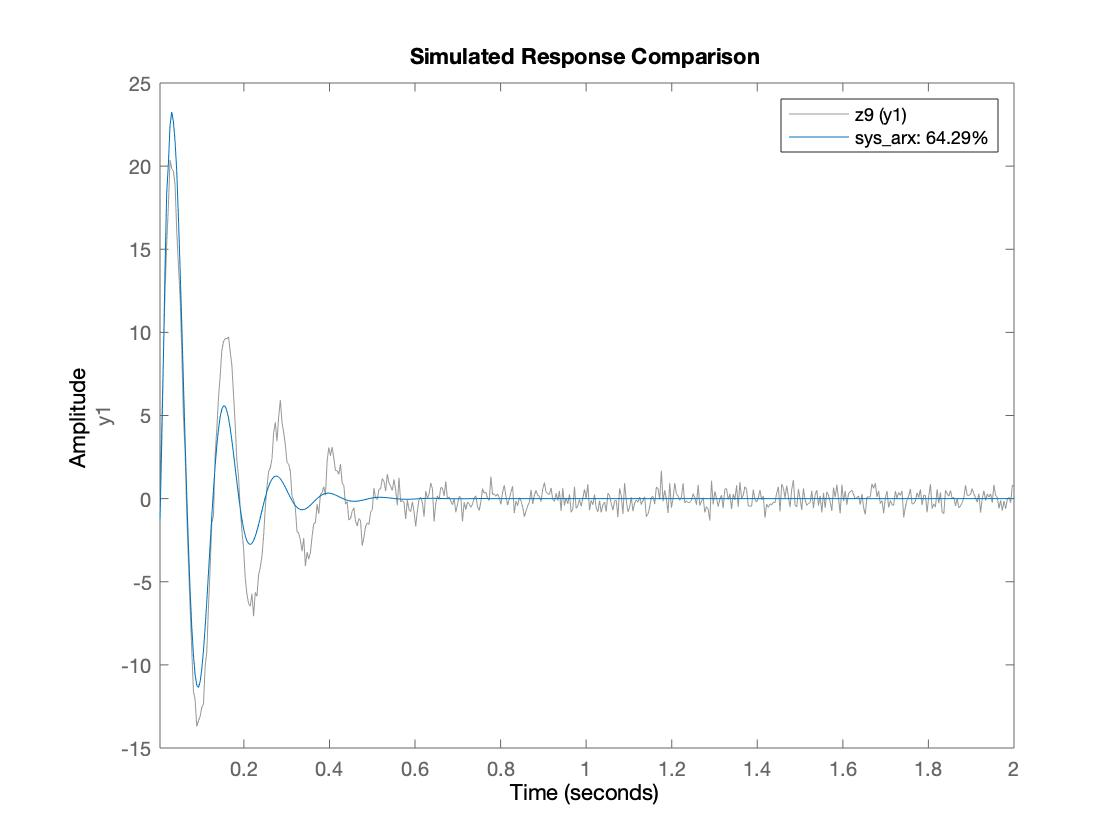
\includegraphics[width = 3in]{control-and-learning/linear-dynamic/graphicx/simulated-response-ARX-model-n=5.jpg}}
\subfigure[nx = 5]{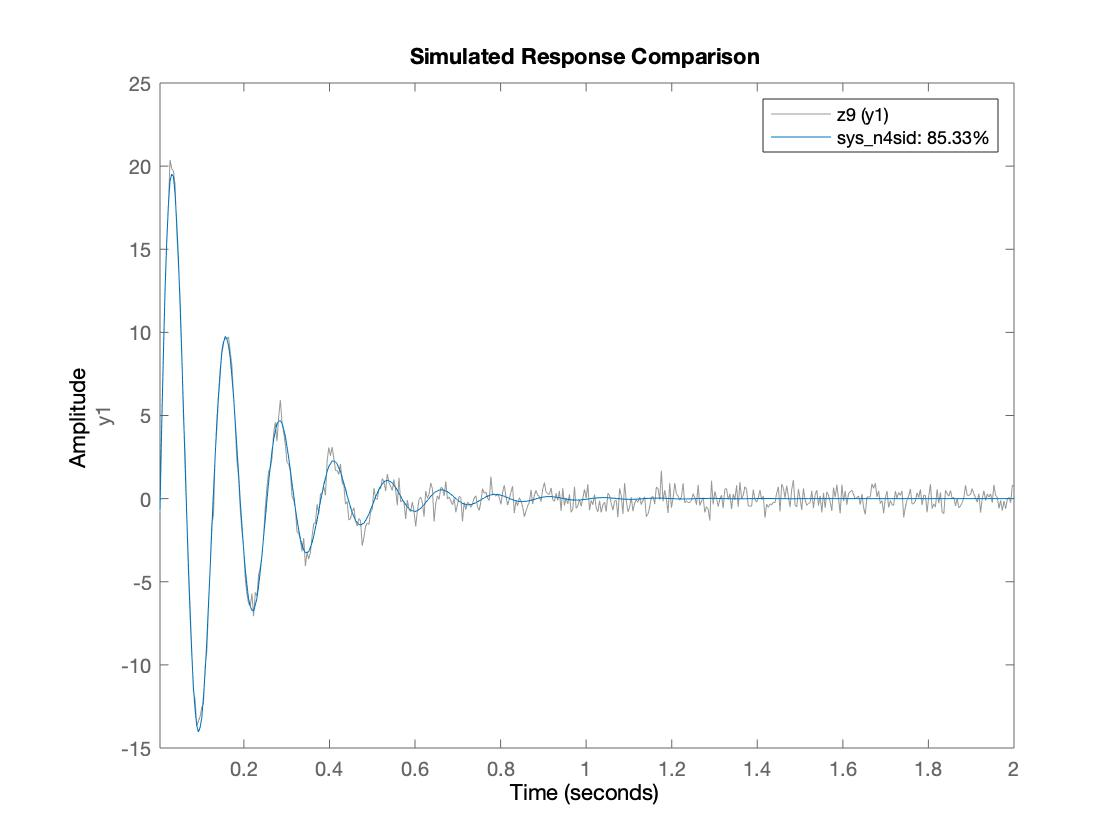
\includegraphics[width = 3in]{control-and-learning/linear-dynamic/graphicx/simulated-response-N4SID-model-n=5.jpg}}\\
\subfigure[nx = 10]{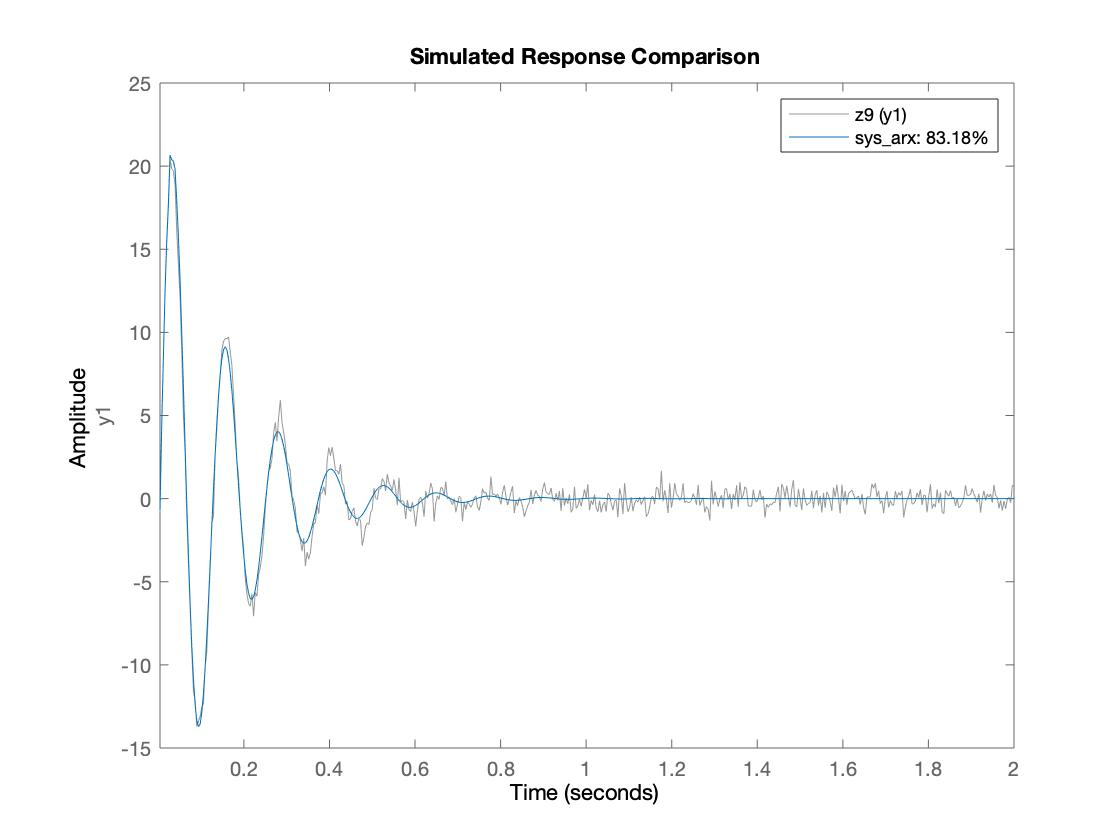
\includegraphics[width = 3in]{control-and-learning/linear-dynamic/graphicx/simulated-response-ARX-model-n=10.jpg}}
\subfigure[nx = 10]{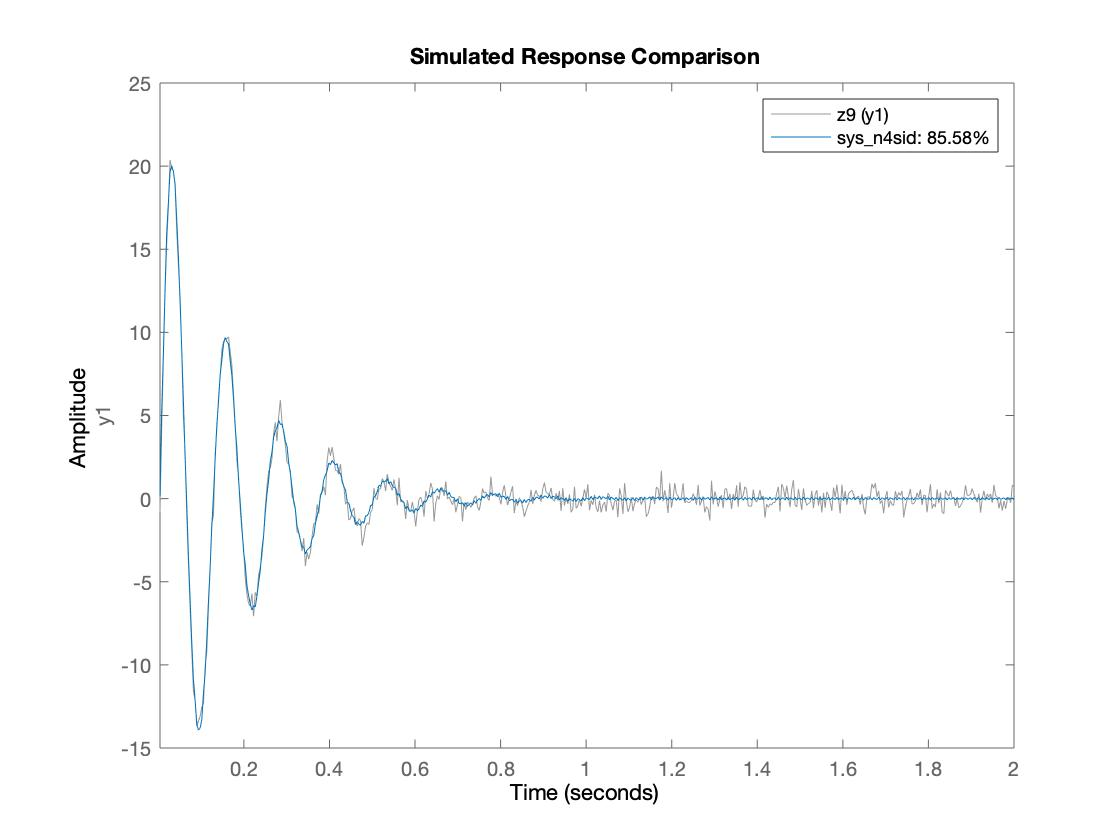
\includegraphics[width = 3in]{control-and-learning/linear-dynamic/graphicx/simulated-response-N4SID-model-n=10.jpg}}\\
\subfigure[nx = 20]{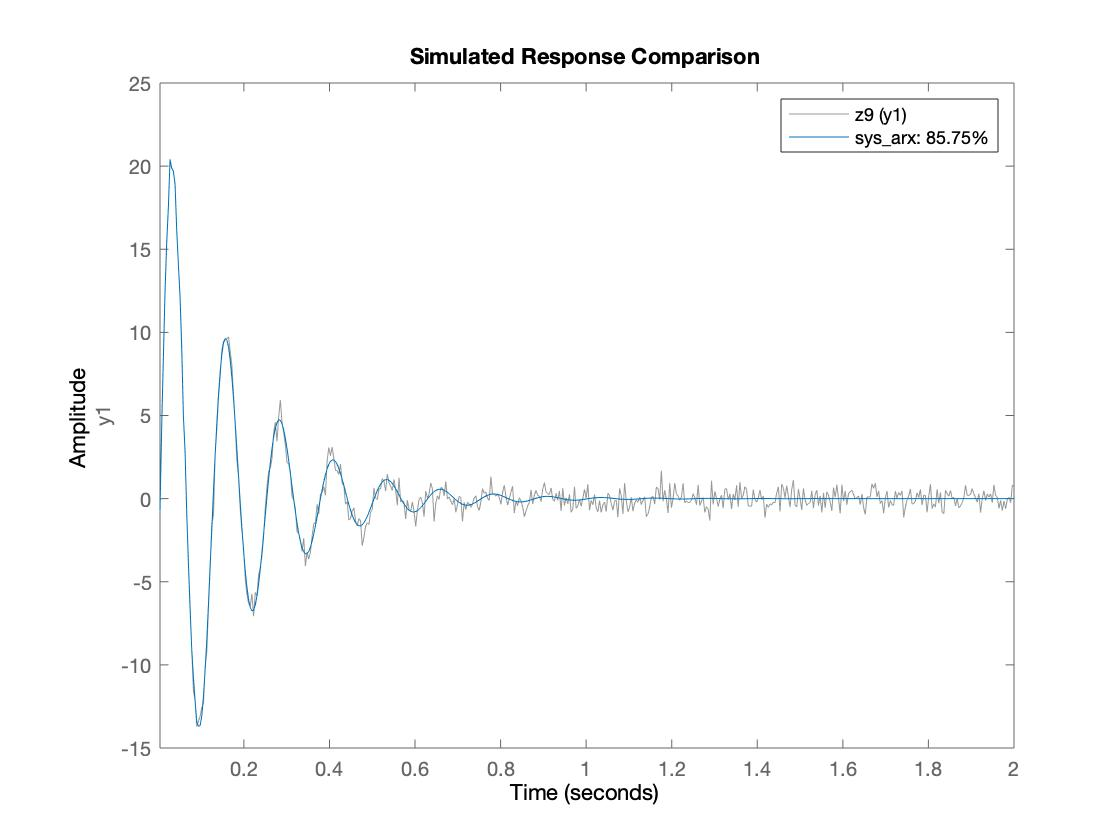
\includegraphics[width = 3in]{control-and-learning/linear-dynamic/graphicx/simulated-response-ARX-model-n=20.jpg}}
\subfigure[nx = 20]{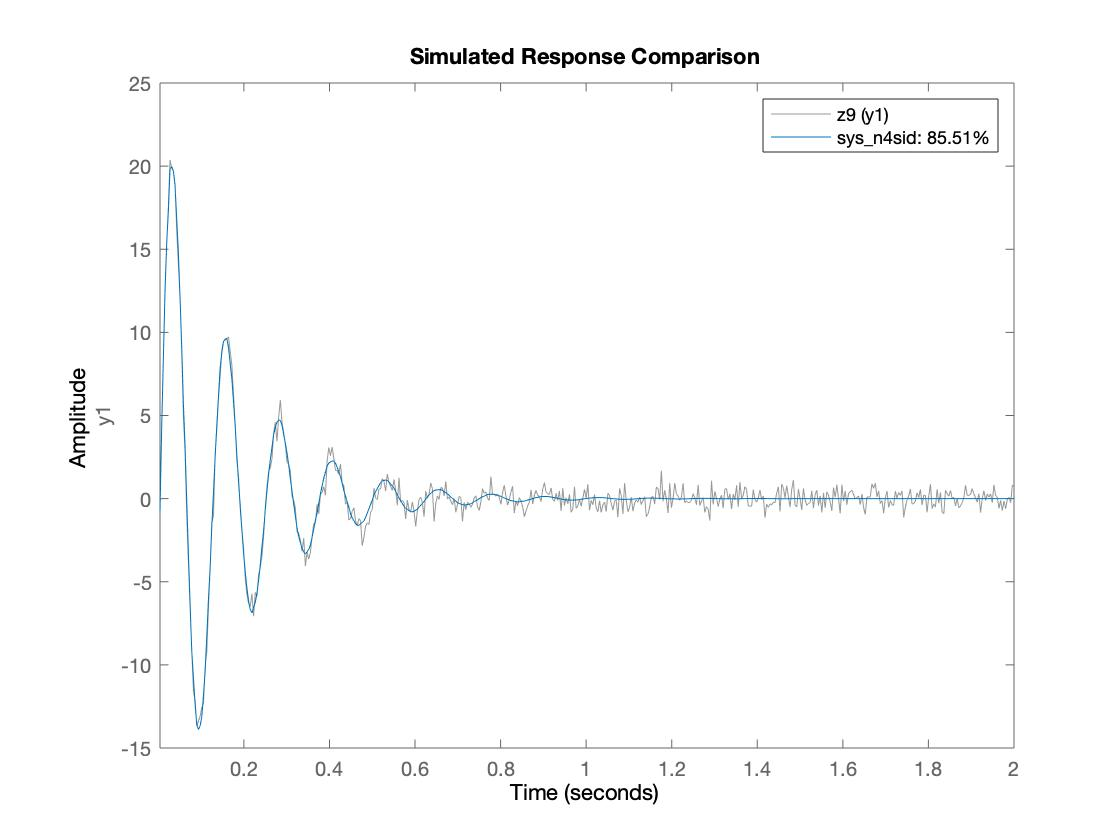
\includegraphics[width = 3in]{control-and-learning/linear-dynamic/graphicx/simulated-response-N4SID-model-n=20.jpg}}\\
\end{figure}

\printbibliography


\end{document}






